\chapter{複雑系としての社会契約}
「倫理ある商取引ゲーム」において、倫理という限定合理性を仮定した上で商取引システムのインセンティブ設計を行えば、
プレイヤーの構成によっては不正が防止され、商取引契約の内容が果たされるようになることがわかった。
本章では、この商取引契約の内容に焦点を当て、これまで外部の強制執行力として存在が仮定されていた「商取引システム」を、
ある集団の成員が構成する複雑系の内部で自己組織化されたシステムとして再現する商取引契約の内容について提案し、
マルチエージェントシミュレーションによって、商取引システムが存在しない場合でも、社会契約が成立しうることを示す。

\section{本章で取り組む問題}
本章では先の章で扱った「倫理ある商取引ゲーム」において、外部の強制執行力として存在が仮定されていた「商取引システム」が存在しない場合でも、
プレイヤーの構成によって「商取引ゲーム」の不正を防止することが可能であるかという問いに取り組む。

\section{本章で検証する仮説}
商取引システムが存在する場合に、商取引契約を履行させることが可能であるとする。
このとき、各プレイヤーが商取引システムと同様の役割を演じその正当性を保証する商取引契約を結ぶことができれば、
外部の強制執行力としての商取引システムが存在せずとも相互監視の元で商取引ゲームで不正を防止し続けることが可能となるだろう。

\section{提案手法}
先の仮説を検証するためには、各プレイヤーが商取引システムの役割を正しく演じる商取引契約の内容を記述し、
その商取引契約の履行を約束する「商取引ゲーム」を繰り返した結果、
全てのプレイヤーが「商取引ゲーム」で不正を行えない状態になりうることを示す必要がある。

ここで、「商取引システム」とはどういったシステムであったかに立ち返ると、
「商取引システム」とは、各プレイヤーの初期の通貨保有量と保存された各時刻の商取引の記録から、
各プレイヤーの通貨保有量を一意に決定するシステムである。
それ故、初期の通貨保有量と保存された各時刻の商取引の記録が全てのプレイヤーで一致しているとき、
全てのプレイヤーが商取引システムが正しく動作しているといえる。

それを実現するためには、各プレイヤーが保存している過去の商取引の記録を互いに確認し合い、
差異が生じた場合に全てのプレイヤーに「失敗」を報告する商取引契約の内容を記述すればよい。

そこで、本章では下記のような『「商取引システム」を自己組織化する商取引契約』を提案し、
先の仮説が成り立つかを検証する。

\subsection{「商取引システム」を自己組織化する商取引契約}
\begin{description}
  \item[step 1] 時刻tを0とする。
  \item[step 2] プレイヤーの人数と各プレイヤーが初期に保有する通貨の量を任意に決定する。
  \item[step 3] N人のプレイヤーが互いに全てのプレイヤーとsellerとbuyerの2つの役割で商取引ゲームを行う周期ある順序を決定する。この周期の長さはN*N-1となる。
  \item[steo 4] 時刻tを1進める。
  \item[step 5] step3で決定した順序にに基づいて時刻tのsellerとbuyerを決定する。
  \item[step 6] 自分が$seller$ならば、時刻$\max\{0, t-n*(n-1)\}$から時刻$t$までに報告された商取引ゲームの記録のうち、
    報告者がその商取引ゲームの記録のbuyerと一致するものを全てbuyerに送信する。
  \item[step 7] 自分が$buyer$ならば、$seller$から受け取った商取引ゲームの記録をメモする。
    この際、記録する商取引の記録の報告者を$seller$に書き換える。
  \item[step 8] 自分が$buyer$ならば、時刻$\max\{0, t-2*n*(n-1)\}$から時刻$\max{0, t-n*(n-1)}$までの各時刻について、
    メモされた商取引の記録のうち自身が報告者の記録はそのまま商取引システムに保存する。
    それ以外の記録は、「成功」と「失敗」のそれぞれの報告者について、自身の所有する商取引システムの通貨保有量の総和をとり、
    大きい方の結果を採用して商取引システムに保存する。
  \item[step 9] 自身が$buyer$ならば、支持する商取引の記録を自身の所有する商取引システムに保存する。
  \item[step 10] 自身が$buyer$ならば、時刻$\max\{0, t-2*n*(n-1)\}$から時刻$\max{0, t-n*(n-1)}$までの各時刻について、
    自身の所有する商取引システムに保存した商取引の記録と、報告者が$seller$であるメモされた商取引の記録を比較し、
    全てが一致するする場合には「成功」を1つでも一致しない場合は「失敗」を全てのプレイヤーに報告する。
  \item[step 11] 全てのプレイヤーは$buyer$から受けた商取引の記録をメモする。この際、商取引の記録の報告者を$buyer$に書き換える。
  \item[step 12] step4に戻る。
\end{description}

\section{実験方法}
  明確に商取引契約を履行しているプレイヤーとそうでないプレイヤーを分けるために、
  『「商取引システム」を自己組織化する商取引契約』の内容を一部改変した「実験用の商取引契約」と8タイプのエージェントを用意する。

  誠実なエージェント(エージェントタイプA)の人数Kが0〜7までの場合でそれぞれ8000回づる下記の施行を繰り返す。

  \begin{itemize}
    \item[step 1] タイプAのエージェントの人数がKになり、残りがB~Hで構成されるような8体のエージェントをランダムに用意する。
    \item[step 2] 初期の各プレイヤーの通貨保有量を8とし、時刻$t$が1120になるまで実験用の商取引契約に基づく商取引ゲームを繰り返す。 
    \item[step 3] 時刻$t=1120$まで下記の施行を繰り返し、各エージェントの所有する商取引システムが有効だと判断したについて、
    報告された成功率と真の成功率を記録する。
  \end{itemize}

  \subsection{実験用の商取引契約}
    \begin{description}
      \item[step 6] 自分が$seller$ならば、時刻$\max\{0, t-n*(n-1)\}$から時刻$t$までに報告された商取引ゲームの記録のうち、
        報告者がその商取引ゲームの記録のbuyerと一致するものを全てbuyerに送信する。
        その際、メッセージに「UTC」の文字列を追記して送信する。
      \item[step 10] 自身が$buyer$ならば、時刻$\max\{0, t-2*n*(n-1)\}$から時刻$\max{0, t-n*(n-1)}$までの各時刻について、
        自身の所有する商取引システムに保存した商取引の記録と、報告者が$seller$であるメモされた商取引の記録を比較し、
        全てが一致するする場合には「成功」を1つでも一致しない場合は「失敗」を全てのプレイヤーに報告する。
        ただし、step7で$seller$から送られてきたメッセージが「UTC」でない場合は、全てが一致していても「失敗」を報告する。
    \end{description}

  \subsection{8種類のエージェント}
    \begin{itemize}
      \item タイプA…step6で「UTC」を送り、step10で「UTC」が送られてきた場合は「成功」、それ以外の場合は「失敗」を報告する
      \item タイプB…step6で「UTC」を送り、step10で「UTC」が送られてきた場合は「成功」、それ以外の場合は「成功」を報告する
      \item タイプC…step6で「UTC」を送り、step10で「UTC」が送られてきた場合は「失敗」、それ以外の場合は「成功」を報告する
      \item タイプD…step6で「UTC」を送り、step10で「UTC」が送られてきた場合は「失敗」、それ以外の場合は「失敗」を報告する
      \item タイプE…step6で「JST」を送り、step10で「JST」が送られてきた場合は「成功」、それ以外の場合は「失敗」を報告する
      \item タイプF…step6で「JST」を送り、step10で「JST」が送られてきた場合は「成功」、それ以外の場合は「成功」を報告する
      \item タイプG…step6で「JST」を送り、step10で「JST」が送られてきた場合は「失敗」、それ以外の場合は「成功」を報告する
      \item タイプH…step6で「JST」を送り、step10で「JST」が送られてきた場合は「失敗」、それ以外の場合は「失敗」を報告する
    \end{itemize}

\section{評価}
サンプリングした結果を元に、タイプAのエージェントと自己組織化が成功した割合をプロットすると、
図\ref{compex-system-002}のようになる。この図から、誠実なプレイヤーが6人以上の場合は全てのサンプルで自己組織化に成功していることがわかる。

\begin{figure}[h]
  \begin{tabular}{cc}
    \begin{minipage}[t]{1\hsize}
      \centering
      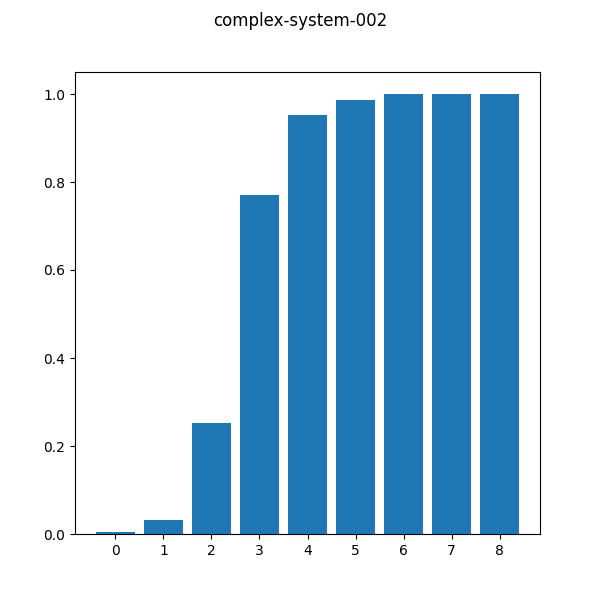
\includegraphics[keepaspectratio, width=1\linewidth]{./05_complex-system/complex-system-002.png}
      \caption{誠実なエージェントの数と自己組織化に成功した割合}
      \label{compex-system-002}
    \end{minipage}
  \end{tabular}
\end{figure}
